\subsection{Error Estimation and Refinement}

Instead of considering a sequence of uniformly refined meshes, we want to consider a new algorithm which locally\footnote{On every element of the mesh.} evaluates an error estimator and marks a certain number of elements which will be then refined.

We consider the following local error estimator:
\begin{gather} \label{estimator}
	\eta_K^2 = h_K \lVert f + \Delta u_h \rVert_{0, K}^2 + \frac{1}{2} \sum_{e \in E_K} h_K \lVert \llbracket \underline{\nabla} u_h \rrbracket \rVert_{0, e}.
\end{gather}

In our 1D case we can rewrite \ref{estimator} as it follows\footnote{$K = [x_{n - 1}, x_n]$.}:
\begin{gather}
	\eta_K^2 = h_K \lVert f \rVert_{0, K}^2 + \frac{1}{2} h_K \left[ \lvert \llbracket u_h^\prime \rrbracket (x_{n - 1}) \rvert + \lvert \llbracket u_h^\prime \rrbracket (x_n) \rvert \right].
\end{gather}

By evaluating $\eta_K$ $\forall K \in \Tau_h$, we can then consider an arbitrary number of elements with the highest local error, say the 25\%, and mark these elements. The last step of this algorithm would be, considering all the marked elements, to refine these by adding a new node at their midpoint.

The algorithm should be summarized in the following way:
\begin{description}
	\item[Solve] Solve the FEM problem on the \textit{starting mesh}.
	\item[Estimate] Estimate the local error on every element of the mesh.
	\item[Mark] Mark the element with the highest local error.
	\item[Refine] Refine the marked elements.  
	\item[Repeat] Repeat the algorithm an arbitrary number of times. 
\end{description}

\newpage
\subsection{Reliability}

Let's test the results given by the following theorem on a sequence of uniformly refined mesh. This'll let us test the reliability of the error estimator $\eta$.

\begin{theorem}[Reliability]
	Let $u \in H_0^1(\Omega)$ solution to the Poisson problem and $u_h$ solution to the Lagrangian FEM with a shape regular and quasi-uniform mesh $\Tau_h$. \\
	Then $\exists C$\footnote{$C$ depends only on the mesh $\Tau_h$.} such that:
	\begin{gather}
		\lvert u - u_h \rvert_{1, \Omega} \leq C \eta,
	\end{gather}
	where:
	\begin{gather}
		\eta^2 = \sum_{K \in \Tau_h} \eta_K^2.
	\end{gather}
\end{theorem}

\begin{figure}[!ht]
	\centering
	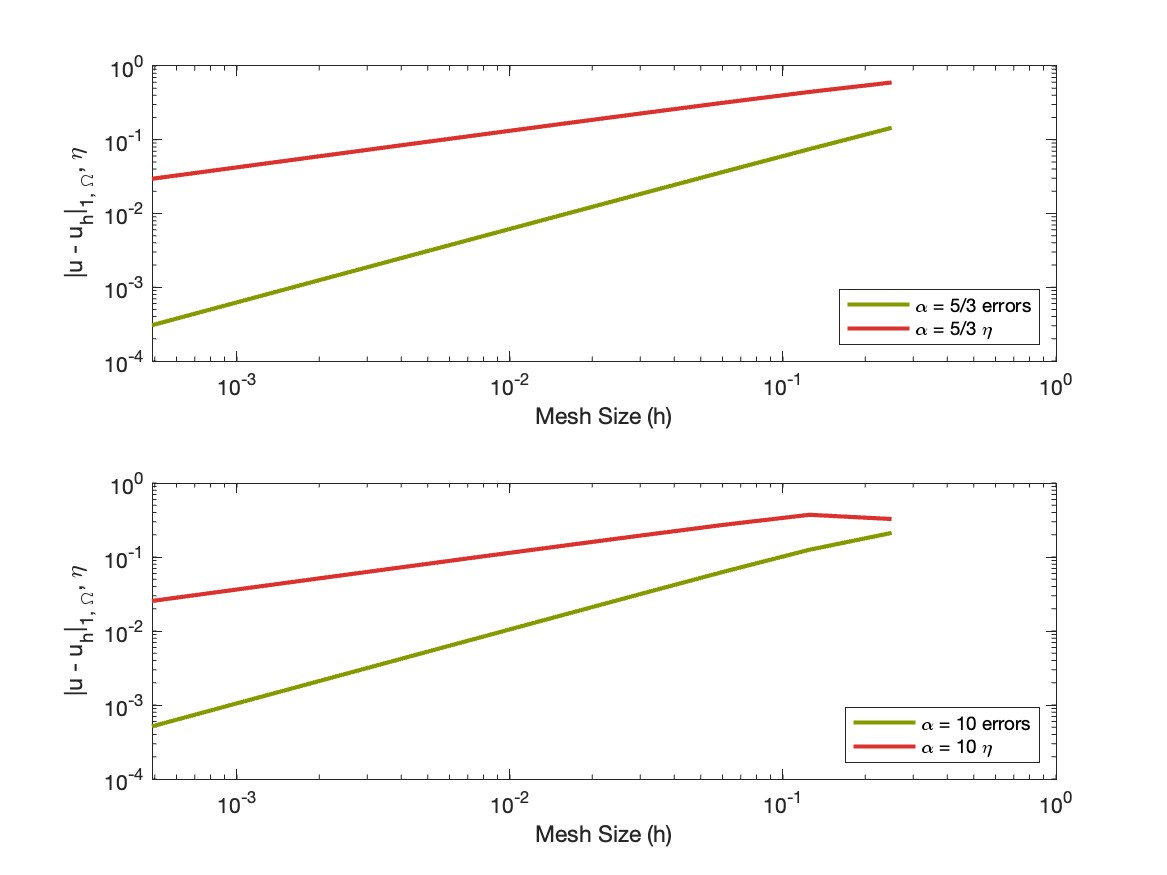
\includegraphics[width=15cm]{reliability.jpg}
	\caption{Comparison between errors and estimator against mesh size.}
\end{figure}

\newpage
\lstinputlisting{../results/reliability.txt}